\documentclass{article}

\usepackage{../preamble}
\standalonetrue

\pagestyle{fancy}
\fancyhf{}
\rhead{Section \thesection}
\lhead{PHYS 304 Lecture 20}
\rfoot{Page \thepage}


\title{PHYS 304 Lecture 20}
\author{Ashtan Mistal}
\date{!!!}

\begin{document}

\ifstandalone
\maketitle
\fi

\graphicspath{{./Lecture20/}}

\subsection{Review of key points from last lecture}

We talked about the relationship of the symmetries that leave the potential function invariant under coordinate transformation, and the degeneracy of energy eigen states: no symmetry, no degeneracy, the more symmetry, the more degeneracy, roughly speaking.

We discussed how our 3D infinite well potential solutions relate to atomic “orbitals” (essentially the magnitude of the distinct eigen \textit{functions}) and the energy of photons emitted by excited atoms (essentially the difference of energy eigen \textit{values }between excited states and lower lying states of the electron).

We discussed how electrons might be induced to make transitions from one “stationary” state to another, via interaction (collisions) with other entities (electrons, photons).

\section{Today}

Find the angular contributions to the solution of the central potential TISE.
Discuss properties of the complete eigen states of the spherically-symmetric potential problem when the potential takes the form $V(\vec{r}) = V(|\vec{r}|) = V(r) \propto \frac{1}{r}$.  (will defer discussion of what approximations go into using $\hat{H}_{hydr. atm.} \approx \frac{\hat{\vec{p}} \cdot \hat{\vec{p}}}{2m} - \frac{e^2}{4 \pi \epsilon_0} \frac{1}{r}$

\subsection{Solving the Schrodinger Equation}

$$
\left.\begin{array}{l}
i \hbar \frac{\partial}{\partial t} \Psi(\vec{r}, t)=-\frac{\hbar^{2}}{2 m} \nabla^{2} \Psi(\vec{r}, t)+\mathrm{V}(x, y, z) \Psi(\vec{r}, t) \\
i \hbar \frac{\partial}{\partial t} \Psi(x, y, z, t)=-\frac{\hbar^{2}}{2 m} \nabla^{2} \Psi(x, y, z, t)+V(x, y, z) \Psi(x, y, z, t)
\end{array}\right]-\nabla^{2} \equiv \frac{\partial^{2}}{\partial x^{2}}+\frac{\partial^{2}}{\partial y^{2}}+\frac{\partial^{2}}{\partial z^{2}}
$$

$$
\begin{aligned}
&i \hbar \frac{\partial}{\partial t} \Psi(\vec{r}, t)=-\frac{\hbar^{2}}{2 m} \nabla^{2} \Psi(\vec{r}, t)+\mathrm{V}(|\vec{r}|) \Psi(\vec{r}, t) \\
&i \hbar \frac{\partial}{\partial t} \Psi(r, \theta, \phi, t)=-\frac{\hbar^{2}}{2 m} \nabla^{2} \Psi(r, \theta, \phi, t)+\mathrm{V}(r) \Psi(r, \theta, \phi, t) \\
&\therefore \nabla^{2}=\frac{1}{r^{2}} \frac{\partial}{\partial r}\left(r^{2} \frac{\partial}{\partial r}\right)+\frac{1}{r^{2} \sin \theta} \frac{\partial}{\partial \theta}\left(\sin \theta \frac{\partial}{\partial \theta}\right)+\frac{1}{r^{2} \sin ^{2} \theta}\left(\frac{\partial^{2}}{\partial \phi^{2}}\right)
\end{aligned}
$$

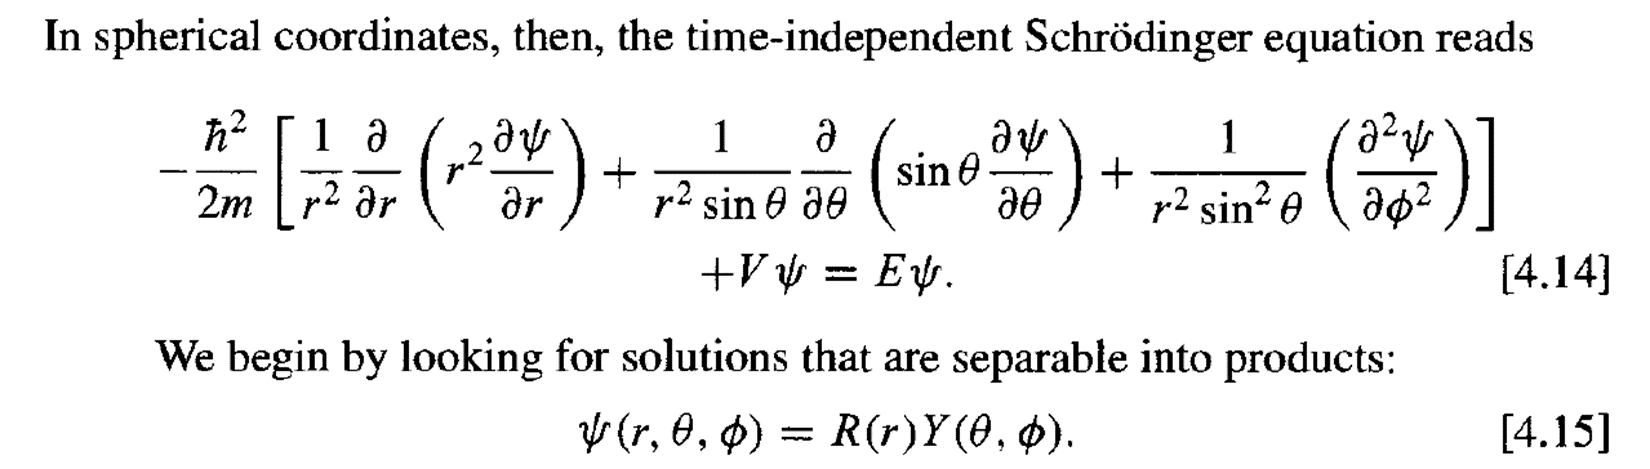
\includegraphics[width = 0.5 \textwidth]{Lecture20/1.png}

$$
\begin{array}{cc}
\left\{\frac{1}{R} \frac{d}{d r}\left(r^{2} \frac{d R}{d r}\right)-\frac{2 m r^{2}}{\hbar^{2}}[V(r)-E]\right\} & \text { The angular equation } \\
+\frac{1}{Y}\left\{\frac{1}{\sin \theta} \frac{\partial}{\partial \theta}\left(\sin \theta \frac{\partial Y}{\partial \theta}\right)+\frac{1}{\sin ^{2} \theta} \frac{\partial^{2} Y}{\partial \phi^{2}}\right\}=0 . & \sin \theta \frac{\partial}{\partial \theta}\left(\sin \theta \frac{\partial Y}{\partial \theta}\right)+\frac{\partial^{2} Y}{\partial \phi^{2}}=-l(l+1) \sin ^{2} \theta Y \\
\frac{1}{R} \frac{d}{d r}\left(r^{2} \frac{d R}{d r}\right)-\frac{2 m r^{2}}{\hbar^{2}}[V(r)-E]=l(l+1) ; & \left\{\frac{1}{\Theta}\left[\sin \theta \frac{d}{d \theta}\left(\sin \theta \frac{d \Theta}{d \theta}\right)\right]+l(l+1) \sin ^{2} \theta\right\}+\frac{1}{\Phi} \frac{d^{2} \Phi}{d \phi^{2}}=0 . \\
\frac{1}{Y}\left\{\frac{1}{\sin \theta} \frac{\partial}{\partial \theta}\left(\sin \theta \frac{\partial Y}{\partial \theta}\right)+\frac{1}{\sin ^{2} \theta} \frac{\partial^{2} Y}{\partial \phi^{2}}\right\}=-l(l+1) . & \frac{1}{\Theta}\left[\sin \theta \frac{d}{d \theta}\left(\sin \theta \frac{d \Theta}{d \theta}\right)\right]+l(l+1) \sin ^{2} \theta=m^{2} \\
\frac{1}{\Phi} \frac{d^{2} \Phi}{d \phi^{2}}=-m^{2} .
\end{array}
$$

$$\Phi(\phi) = e^{i m \phi}, \quad m = 0,\pm 1, \pm 2,...$$

$$\Phi(\phi + 2 \pi) = \Phi(\phi)$$

The $\theta$ equation may not be so familiar:

$$\sin (\theta) \frac{d}{d \theta} \left( \sin(\theta) \frac{d \Theta}{d \theta} \right) = \left[ l(l+1) \sin^2 (\theta) - m^2 \right] \Theta = 0$$


The solution is:

$$\Theta(\theta) = A P_l^m (\cos \theta)$$

where $P_l^m$ is the \textbf{associated Legendre function, defined by}

$$P_l^m(x) = (1-x^2)^{|m|/2} \left( \frac{d}{dx} \right)^{|m|} P_l(x)$$

This also implies maximum $|m| = 1$.

$$P_l(x) = \frac{1}{2^l l!} \left( \frac{d}{dx} \right)^l (x^2 - 1)^l$$

This implies $l$ must be a non-negative integer for the derivative to make sense. 


\subsection{Full angular solution}


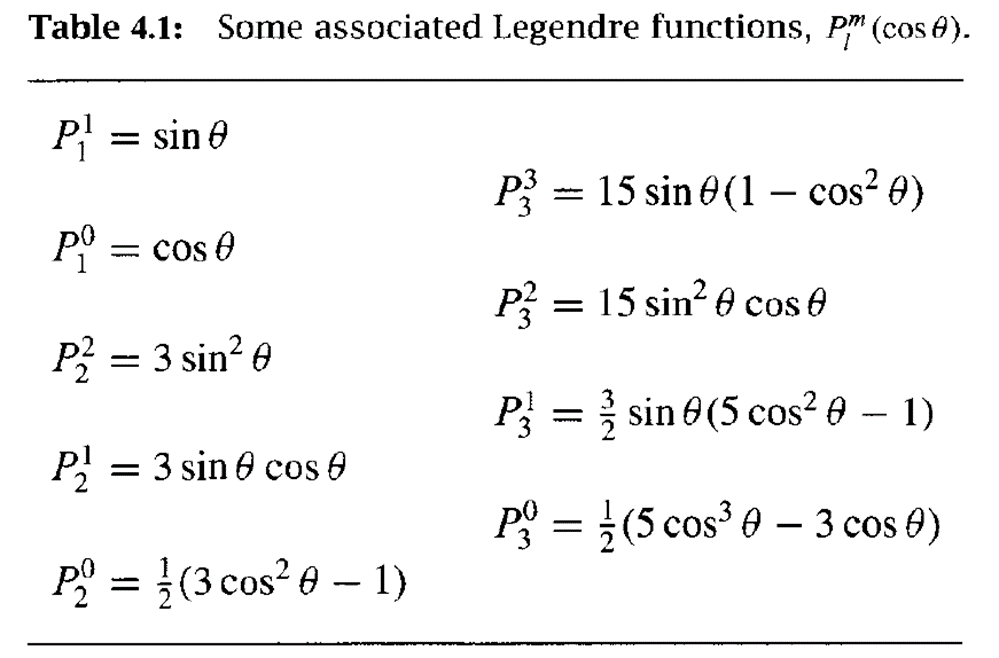
\includegraphics[width=  0.6 \textwidth]{Lecture20/2.png}

$$Y_{l}^{m}(\theta, \phi)=\epsilon \sqrt{\frac{(2 l+1)(l-|m|) !}{4 \pi} \frac{(l-|m|) !}{(l+|m|) !}} e^{i m \theta} P_{l}^{m}(\cos \theta)$$

$\epsilon=(-1)^{m}$ for $m \geq 0$ and $\epsilon=1$ for $m \leq 0$

$$\int_{0}^{2 \pi} \int_{0}^{\pi}\left[Y_{l}^{m}(\theta, \phi)\right]^{*}\left[Y_{l^{\prime}}^{m^{\prime}}(\theta, \phi)\right] \sin (\theta) d \theta d \phi=\delta_{l l^{\prime}} \delta_{m m^{\prime}}$$

Table 4.2: The first few spherical harmonics, $Y_{l}^{m}(\theta, \phi)$.
$$
\begin{aligned}
Y_{0}^{0} &=\left(\frac{1}{4 \pi}\right)^{1 / 2} & & Y_{2}^{\pm 2}=\left(\frac{15}{32 \pi}\right)^{1 / 2} \sin ^{2} \theta e^{\pm 2 i \phi} \\
\hline
Y_{1}^{0} &=\left(\frac{3}{4 \pi}\right)^{1 / 2} \cos \theta & Y_{3}^{0} &=\left(\frac{7}{16 \pi}\right)^{1 / 2}\left(5 \cos ^{3} \theta-3 \cos \theta\right) \\
\hline
Y_{1}^{\pm 1} &=\mp\left(\frac{3}{8 \pi}\right)^{1 / 2} \sin \theta e^{\pm i \phi} & Y_{3}^{\pm 1} &=\mp\left(\frac{21}{64 \pi}\right)^{1 / 2} \sin \theta\left(5 \cos ^{2} \theta-1\right) e^{\pm i \phi} \\
\hline
Y_{2}^{0} &=\left(\frac{5}{16 \pi}\right)^{1 / 2}\left(3 \cos ^{2} \theta-1\right) & Y_{3}^{\pm 2} &=\left(\frac{105}{32 \pi}\right)^{1 / 2} \sin ^{2} \theta \cos \theta e^{\pm 2 i \phi} \\
\hline
Y_{2}^{\pm 1} &=\mp\left(\frac{15}{8 \pi}\right)^{1 / 2} \sin \theta \cos \theta e^{\pm i \phi} & Y_{3}^{\pm 3} &=\mp\left(\frac{35}{64 \pi}\right)^{1 / 2} \sin ^{3} \theta e^{\pm 3 i \phi}
\end{aligned}
$$

\subsection{Pause}

How do any of these spherical harmonic functions depend on the exact form of the radially symmetric potential?

\textbf{They don’t, explicitly.  They will indirectly connect via the shared constant identified in the first separation of variables step in the derivation, but there is no explicit V(r) dependence in these spherical harmonics.
}

Pause: what do we know (and what do we not know) so far about the solutions of the time-independent SE for a particle that experiences a spherically symmetric potential?  

We know precisely that their theta and phi dependence is constrained to functions with shapes that depend only on two integers, l and m, where for any $l \geq 1$, there are $2l+1$ allowed values of $m: -l, -l+1,..0,1,...l$, and the total number of nodes, split between the theta and phi degrees of freedom is equal to l, and the number of nodes in the phi degree of freedom is $|m|$.

We know nothing about the radial part of the solution.

\subsection{Radial Part of the Solution}

\
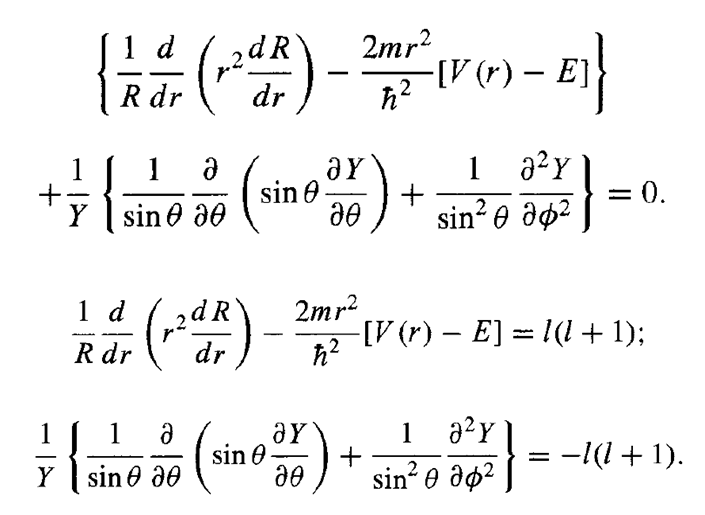
\includegraphics[width = 0.6 \textwidth]{Lecture20/3.png}

Bottom function still as a function of V(r)


The third line leads to the following:

$$- \frac{\hbar^2}{2m} \frac{d^2 u}{dr^2} + \left[ V + \frac{\hbar^2}{2m} \frac{l(l+1)}{r^2} \right] u = Eu$$

where $u(r) \equiv r R(r)$

Before we go any further, what do we need to know?

$$V(r) = - \frac{e^2}{4 \pi \epsilon_0} \frac{1}{r}$$

The hydrogen atom, specifically for the Coulomb potential.  

Note that they are connected only by l, not m. 

For bound states, $E < 0$, so $\kappa$ is real. Dividing Equation 4.53 by $E$, we have the following:

$$\frac{1}{\kappa^2} \frac{d^2 u}{dr^2} = \left[ 1 - \frac{me^2}{2 \pi \epsilon_0 \hbar^2 \kappa} \frac{1}{\kappa r} + \frac{l(l+1)}{\kappa^2 r^2} \right] u$$

where $\kappa = \frac{\sqrt{-2mE}}{\hbar}$

With $\rho \equiv \kappa r$, and $\rho_0 = \frac{me^2}{2m\epsilon_0 \hbar^2}$:

$$\frac{d^2 u}{d \rho^2} = \left[ 1 - \frac{\rho_0}{\rho} + \frac{l(l+1)}{\rho^2} \right] u$$

As $\rho \to \infty$, 

$$\frac{d^2 u}{d \rho^2} = u; \quad u(\rho) = Qe^{- \rho} + Be^\rho; \quad u(\rho) ~ Ae^{- \rho}$$

As $\rho \to 0$, 

$$\frac{d^2}{d \rho^2} = \frac{l(l+1)}{\rho^2}; \quad u(\rho) = C \rho^{l+1} + D \rho^{- l}, \quad u(\rho) ~ C \rho^{l+1}$$

Similar to the harmonic oscillator, where we assumed a functional form that includes a polynomial, and do a power series expansion of that polynomial to get a recursion formula for it’s coefficients. Just like the harmonic oscillator, they can’t be arbitrarily large, so specific sets of coefficients dictated by a requirement for there to be a maximum power in a given polynomial solution.  $j=0$ corresponds to the constant, $j=1$ to the linear term in rho, etc.


$$u(\rho) = \rho^{l+1} e^{-p} v(\rho) \quad \& \quad \frac{d^2 u}{d \rho^2} = \left[ 1 - \frac{\rho_0}{\rho} + \frac{l(l+1)}{\rho^2} \right] u$$

$$\therefore \rho \frac{d^2 v}{d \rho^2} + 2(l+1-\rho) \frac{dv}{d \rho} + \left[ \rho_0 - 1(l+1) \right] v = 0$$

Does this remind you of any other equation we have encountered?

Assume the following:

$$v(\rho) = \sum_{j=0}^\infty a_j \rho^j$$

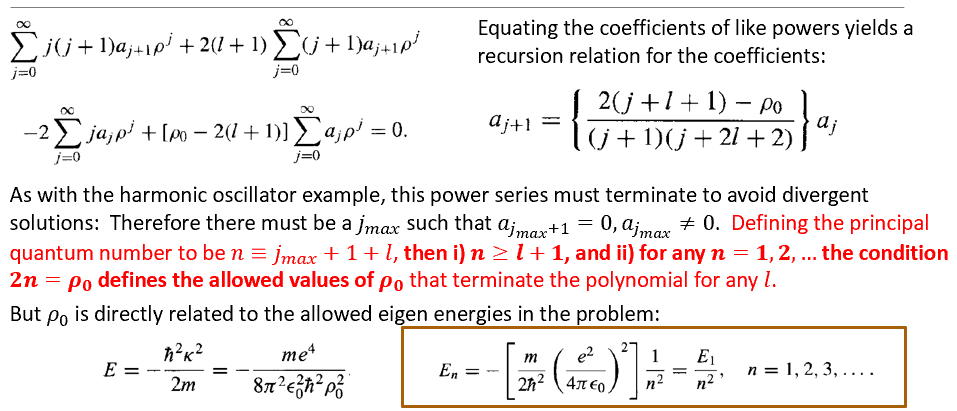
\includegraphics[width = 0.9 \textwidth]{Lecture20/4.png}

Note, $n=N+l$ (Eqn. 2.67) where $N$ is the order of the radial polynomial in the expansion, so $N-1$ is equal to the number of nodes in the radial function $R$, which is therefore $= n-l-1$. Check with figure 4.7

\section{The full set of eigen functions ($n, \ell, m)$}

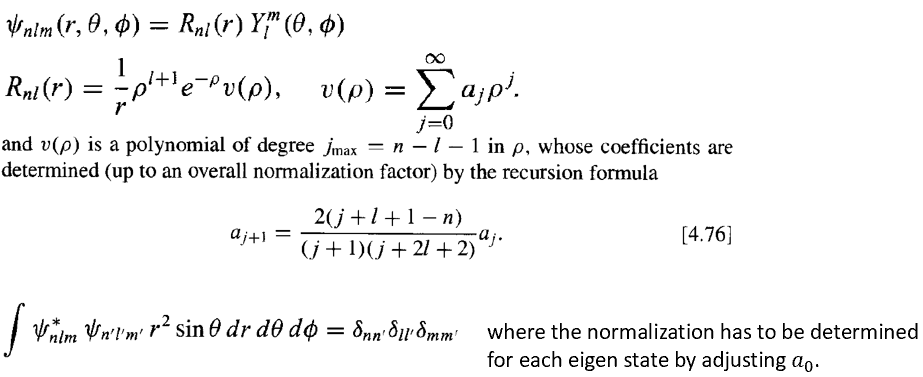
\includegraphics[width = 0.9 \textwidth]{Lecture20/5.png}

You can always look up or numerically evaluate the actual special functions, but the key things you must understand are the relationships/dependencies between the integers $n, l,$ and $m$, the associated degeneracies, and the number of nodes in each of the degrees of freedom. 

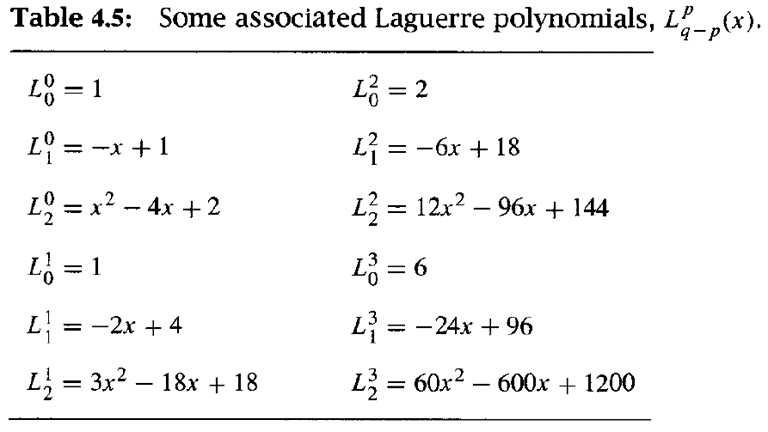
\includegraphics[width = 0.5 \textwidth]{Lecture20/6.png}


\end{document}